\chapter{Testing}

\section{Transducer Device}
As all the functions provided by the transducer device are part of the overall system, the transducer device actually build as demonstration device is tested implicitly in the system tests. This section only covers additional tests that do not directly regard the usability of the demonstration device.

\subsection{Embedded Software}
Most parts of the embedded system software will be tested implicitly in the system testing part, but there are some specific features included in the software that need to be tested separately as they are not used in the demonstration device.

\paragraph{Using an SRAM buffer for resending}
This feature was tested on an Arduino Due microcontroller board as this board is equipped with a higher amount of SRAM allowing the message to be stored in SRAM. At the same time it is a board that does not contain EEPROM and therefore needs to use SRAM or Flash if a resend feature should be available. The only code modifications necessary in comparison to the demonstration device are commenting out the EEPROM\textunderscore RESEND define and defining SRAM\textunderscore RESEND. This system was only tested in order to show the software capability to resend data saved in SRAM. The function has been found to work without any problems.

\paragraph{Using a Hardware Serial for the GPS module}
For this test an Arduino Due has been used as this board contains four hardware serial ports. The software modification needed for this change is commenting out the GPS\textunderscore SOFTWARE\textunderscore SERIAL define and defining GPS\textunderscore SERIAL as the serial port used. There were no problems discovered during this test.

\paragraph{Fault Behavior (resending)}
As the system normally does not produce fault conditions triggering the transducer device to leverage its resending capabilities, this feature is tested separately. There were some test cases created used to test the resending behavior of the transducer demonstration device (which is using the EEPROM as a resending buffer):
\begin{itemize}
\item The pin used transfer information from the Bluetooth module to the Arduino was disconnected. A resend every 5 seconds is expected.
\item The trigger is pushed while the Bluetooth function is disabled in the app. When Bluetooth is reactivated, receiving the message on the Android device should take at most 5 seconds.
\item The resend option in the application software settings is used. The occurence of two data records distinct only by the receive time is expected.
\item The trigger is pushed while Bluetooth is switched off on the Android device. After the measurement, the transducer is turned off. While the transducer is turned off, Bluetooth and the app are activated on the Android device. The expected result is receiving the data as soon as the transducer is turned on.
\end{itemize}

All these tests were carried out and the expected behavior was fulfilled in all cases.

\subsection{Energy Consumption}
As a multitude of different sensors and microcontrollers might be used in the transducer platform, no conclusive statement regarding the energy consumption can be made. However the energy consumption can be probed using the demonstration device described in section \ref{p:demonstration_device}. The demonstration device allows two modes of operation including and excluding the GPS receiver and it's active antenna. The energy consumption has been measured feeding the system through the linear voltage regulator and feeding it directly inputting 3.3 V into the regulated voltage part. Even though current spikes might be observed while searching for Bluetooth devices, reading sensor values and reading or writing EEPROM, the major factor in the system is considered to be standby current draw. Recording the current and voltage output of a HAMEG Instruments HM8143 power supply some values power consumption data was acquired for the whole system and some of its most exposed parts. During all the measurements, each input channel was smoothed by a 1000 $\mu F$ capacitor inserted in the input channels next to the main consumers (the GPS module and the Arduino board).

The standby current can be considered mostly stable and the averages recorded after the startup phase were:
\begin{center}
  \begin{tabular}{ | c | c |}
    \hline
    Arduino Microcontroller, Sensors and Bluetooth module (connected) & 7.7 mA \\ \hline
    GPS module without external antenna & 22.0 mA \\ \hline
    GPS module including external antenna &  31.9 mA \\
    \hline
  \end{tabular}
\end{center}

The data recorded for the GPS module and the antenna approximately coincide to the values stated in the documentation (20 mA for the module, see \cite{AdaUltGPS} and 10 mA for the antenna, see \cite{ExtAnt}).

On startup and while measure data is acquired and sent, the power consumption is somewhat higher, the current draw of the basic system with the GPS connected to a different channel during the operations is shown in figure \ref{fig:startup_current} and figure \ref{fig:send_current} 

\begin{figure*}[ht]
\centering
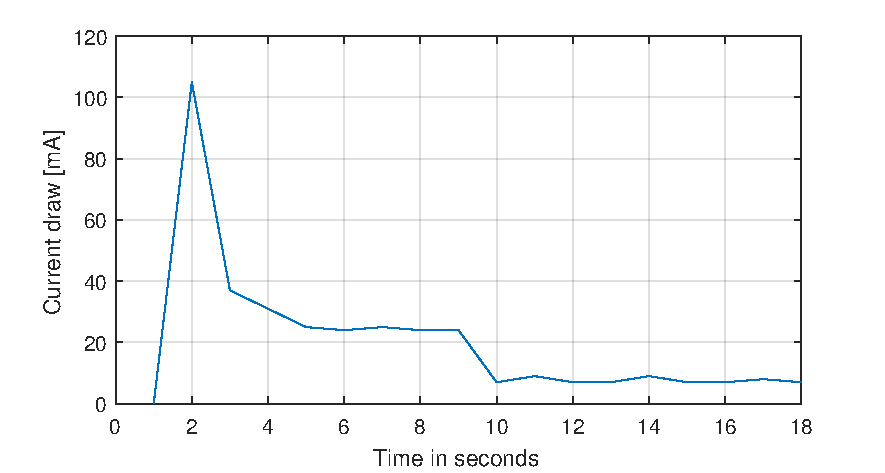
\includegraphics[width=1.0\textwidth]{src/start_current.pdf}
\caption{Current draw on system startup (without GPS)}
\label{fig:startup_current}
\end{figure*}

\begin{figure*}[ht]
\centering
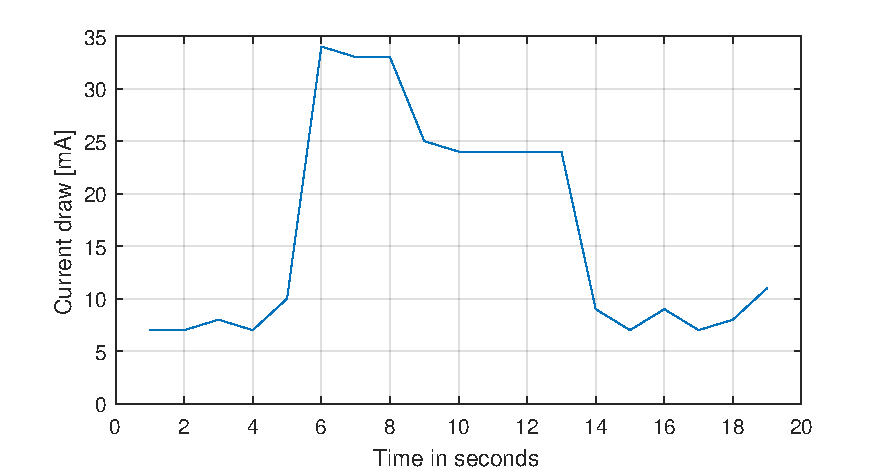
\includegraphics[width=1.0\textwidth]{src/send_current.pdf}
\caption{Current draw after a measurement has been triggered (without GPS)}
\label{fig:send_current}
\end{figure*}

\section{Application Software Testing}
\subsection{Core App Quality}
The application software was tested against the Core Suite test procedure of the Android Core App Quality guidelines (see \cite{CoreAppQ}). The test devices used in this test were the following:
\begin{itemize}
	\item An Ulefone Power running Android 6.0 and patch level September 5th 2016
	\item A Samsung Galaxy S III mini running Android 4.2.2 Jelly Bean
	\item A Sony Xperia Go running Android 2.3.3 Gingerbread
\end{itemize}

The following issues have been uncovered and resolved in the testing phase:
\begin{itemize}
\item A bug has been found which would lead to text in the FirstStartActivity overflowing from the screen on small screens in landscape mode. This bug has been resolved by wrapping the text in a ScrollView.
\item An application crash (NullPointerException) was provoked when a data record was deleted from the application UI and a notification referring this data record was tapped. The issue has been resolved and the user is shown a toast when such a notification is tapped.
\end{itemize}

\subsubsection{Protocol Compliance}
As only a limited number of sensors might be attached to the transducer device and the resources of some Arduino models are rather limited, tests for the protocol compliance of the Android app have been carried out by using a random message generator (which can be found in the digital appendix) and sending the messages from a desktop computer. In order to send the messages, a USB-TTL adapter was connected to the Bluetooth module normally incorporated in the system. The random message generator produces messages structured as defined in the protocol description (it does not alter any parts of the structure) and fills the data fields with random (but valid) data. The number of virtual \emph{sensors} incorporated might be adjusted freely to test the limits of the system. The random message generator is programmed in Matlab R2017a and uses Matlabs native communication capabilities to establish the serial connection.

\subsection{Application Software Performance}
On all devices used in the core app quality test, no unusual lags were experienced during normal operation. Even the Sony Xperia Go which was released in 2012 and currently runs Android 2.3.3 for testing purposes offered acceptable performance in all views.

\subsubsection{Large Data Record Performance}
When the random message generator is used, the number of virtual sensors included in the message can be adjusted arbitrarily. The application software uses a maximum buffer size of two megabytes for incoming messages. This limit is well beyond the limits of the embedded software used in this system but using a different transducer device or redesigning the software to produce the data as a stream (as opposed to sending the data after all data fields have been collected) might lead to larger messages. This limit leads to an approximate hard limit of 12000 sensor data readouts in one message. Using an enlarged buffer, the limits of the application software have been tested up to 20000 sensors in one message.

The performance tests have been carried out on an Ulefone Power smartphone (see \cite{UlePow}). This smartphone runs Android 6.0 Marshmallow on a 64 Bit MTK6753 octa core processor. It is equipped with 3 GB RAM. The application software on this smartphone was temporarily adjusted to use a larger buffer for incoming messages in order to test very large data sets. When the number of included sensors is set to 1000, the applications main list still responds reasonably quick even though the entry for the large data record has a significant scrollable length. The details view for this entry does however expose serious lag while scrolling as this view is not optimized for large amounts of data.

\subsubsection{Performance for Large Numbers of Data Records}
The random message generator can be used to produce a high number of data records. In this test, the same Ulefone Power smartphone has received 2000 data records each containing on average 5.5 sensor readouts. Still having the large data records produced in the previous test in the database, the performance of the app was assessed. While the main list view still performed reasonably well, even when a filter was applied or the sort order changed, starting the map view led to the application hanging and having the Android system show an \emph{Application not Responding} dialog to the user. Even when the dialog was dismissed several times, the map did not show up while all the data records should have been shown. After a filter is set limiting the number of data records shown to less than hundred, the map draws as expected. When the export function is used on the whole data set. there is no immediate response, but the app continues to react. The data is prepared in the background and when the data is ready, the application chooser (or the application chosen by the user) is shown. On the example data set, the time needed to prepare the export is around 45 seconds. The complete comma separated value table generated in this test has a size of around 35 MB. The application database resulting from this test has a total size of 15 MB. 

\subsection{Internationalization}
In order to test the internationalization of the software, it was run having the Android device set to different languages. As the app natively provides two locales, English and German (both without further distiction by country) with English as the primary (and therefore fallback) language, theese were included in the test as EN-US (United States of America) and DE-DE (Germany). Additionally the IT-IT locale was tested as example for a locale using the fallback language. Dates and times are shown in a local format across the app. During this test no unexpected behavior has been found.

\section{System Testing}
As the usefulness of the system derives only from its parts working together, the parts of the system must be tested to work together.

\subsection{Communication between the Transducer and the Android Device}
In order to test the communication between the transducer and the Android device, a USB-TTL adapter was connected to the data lines connecting the Bluetooth module and the Arduino in the transducer demonstration device. During usage, both communication directions were observed. Regarding the communication direction from the Android device to the transducer, during manual testing, the characters detected matched the expected ones according to the protocol exactly. When the button in the app to trigger a measurement was pushed, a device control 1 character was detected, when a message was received correctly, an acknowledgement character was detected when the resend button in the application settings was pressed, a negative acknowledgement was send. Also when the message structure in the other communication direction was destroyed by inserting invalid structures using the USB-TTL adapter, a negative acknowledgement was received. At the same time, the Android Monitor integrated in Android Studio was used to see the defective message which was logged to the Android log by the application software. In the other direction, the data send by the transducer has been intercepted and checked against the data shown in the app. The data received by the app matched the data intercepted as expected.

\subsection{Data Export}
As second part of the system test, data stored in the application was exported to two different cloud storage providers: Microsoft OneDrive and Google Drive. The data was downloaded to a personal computer from these services and the data in the files was manually compared opening the files in a text editor to the data shown in the application software. No alterations of the information were found. The structure of the file also complied to the expectation.

\subsection{External Data Analysis}
\label{subs:externalDataAnalysis}
\subsubsection{Microsoft Excel}
Microsoft Excel for Windows (the 2016 and Office 365 versions; the Mac and iOS versions lack the this feature) includes a 3D map feature that can be used to generate heat maps, 3D bar graphs and other types of geographic data visualization. It also contains a multitude of other functions for data analysis and visualization. Opening the data exported from the GeoSensor app in Excel for Windows (and in this case also on macOS) works straightforward by double-clicking the file if the csv separator and the decimal mark are set according to what Excel expects in the locale chosen. In a German (Germany) locale, Excel expects csv-files to use a comma as decimal mark and a semicolon as separator character. If these are used when exporting the data, there is no need to adjust anything when opening a file exported from GeoSeosor in Excel. The date and time format used in the exported file is understood by Excel without any further adjustments and also the other data is shown as expected. If the file uses a different set of csv separator and decimal mark, data might be imported using Excels data import assistant, this feature however was not tested.

If Excel is target application for data exported, using OneDrive to transfer the files is recommended. When an appropriately formatted csv file is saved in OneDrive, it can also be opened by the Excel App for Android or iOS when a Microsoft online service is used to convert the data to Excel's native data format. Excel for Windows and macOS can natively open .csv-files.

\subsubsection{Matlab}
The .csv data exported from GeoSensor can be imported into Matlab using the graphical import assistant in Matlab. This assistant can generate a function that imports further data files having the same structure without any further interaction. When using the graphical import assistant, the content format for each table column must be set correctly, especially the time columns need to be set to the right format (the date and time format used is \texttt{yyyy-MM-dd HH:mm:ss}). All matlab data analysis and visualization features can then be used on the resulting table. Matlab deployments having access to the Matlab Mapping Toolbox can leverage its capabilities for advanced geographic visualisation. The test data imported into Matlab does match the information visualised in the app and no problems have been found.

\section{Field Testing}
Remembering the initial goals set for the system, a system test has been carried out to show the suitability of the system for a real-world use case. The external encapsulated temperature sensor of the demonstration device has been used to measure the water temperature in different waterbodies around the University of Bremen. The complete workflow tested here includes setting up the system, the data acquisition, on-the-go visualization of the data, transferring the data to a personal computer and analyzing the data using widespread software.

\subsection{System Setup}
The transducer system used in this field test is the demonstration device as described in paragraph \ref{p:demonstration_device}. Air temperature and humidity data have been recorded during the field test, but the focus was laid on water temperatures. There were no modifications made to the transducer system. The Android application software was installed on a Nexus 7 tablet running an operating system based on Android 7.1 Nougat. The tablet does have a GPS receiver, however there is no cellular data connection. For the field tests, the location has been recorded by both the hardware module incorporated in the transducer and the Fused Location Provider on the tablet.

\subsection{Data Acquisition}
In order to reach the sample points used in the field test, the system was transported on a bicycle. The tablet remained on the bicycle luggage rack while the transducer device was taken to the sample points which were often some meters away from the tablet. Water temperature samples can be taken by throwing the encapsulated sensor (which has two-meter cable to the rest of the transducer) into the water. Before the measurements were triggered, an adaption time of 20 s was awaited in order for the sensor electronics to approach the temperature of the surrounding water. During and between the measurements the user interface on the tablet was not used, all measurements were triggered using the physical button on the transducer.

\subsection{On-The-Go Visualization}
\paragraph{Offline}
While offline, the data can be visualized in the list and details views. In the list view, all the measured values can be seen and the measured values visualized can be considered plausible. The locations seen in the details view don't show significant differences between the locations provided by the GPS module attached to the Arduino and the fused location provider on the Android device.

\paragraph{Online}
When an internet connection is available, in addition to the aforementioned features, the map view and reverse geocoding for the position data is avaliable. The map view shows position data matching the actual positions with a error of less than 5 meters.

The reverse geocoding can not resolve actual street addresses for most of the sample points as most of them are located inside a public park in which the footpaths do not have designated names. One of the sample points however was the pond surrounding the Universum science center which has a street address. In this case the address given by the reverse geocoding exactly matched the official address.

\subsection{Data Export}
The data gathered in the field test has been exported to two different cloud storage providers. A version using semicolons as column separators and commas as decimal marks was exported to Microsoft OneDrive. The other version uses commas as column separators and dots as decimal marks was exported to Google Drive.

\subsection{Data Analysis}
Data exported from the field test has been loaded into the application software mentioned in section \ref{subs:externalDataAnalysis}.  

\subsubsection{Microsoft Excel}
The data saved in OneDrive has been opened directly from OneDrive in Microsoft Excel (Office 365 Version as of June 2017 on Windows, macOS, Android and iOS). The mobile (Android and iOS) versions of Excel needed to use a Microsoft online service for data conversion but otherwise opening the files was possible without any problems.

Excels 3D Maps geographic data visualization capabilities were used to plot a 3D bar graph map of the data acquired during the field test. This map can be found in figure \ref{fig:excel_bar_graph}. As the file has been specifically exported for a German Excel version by using commas as decimal marks and semicolon as separator characters, the file could be opened ina German Excel version without any further steps. In order to include 3D maps the file however needed to be saved in Excel's native \texttt{.xlsx} file format.

\begin{figure*}[ht]
\centering
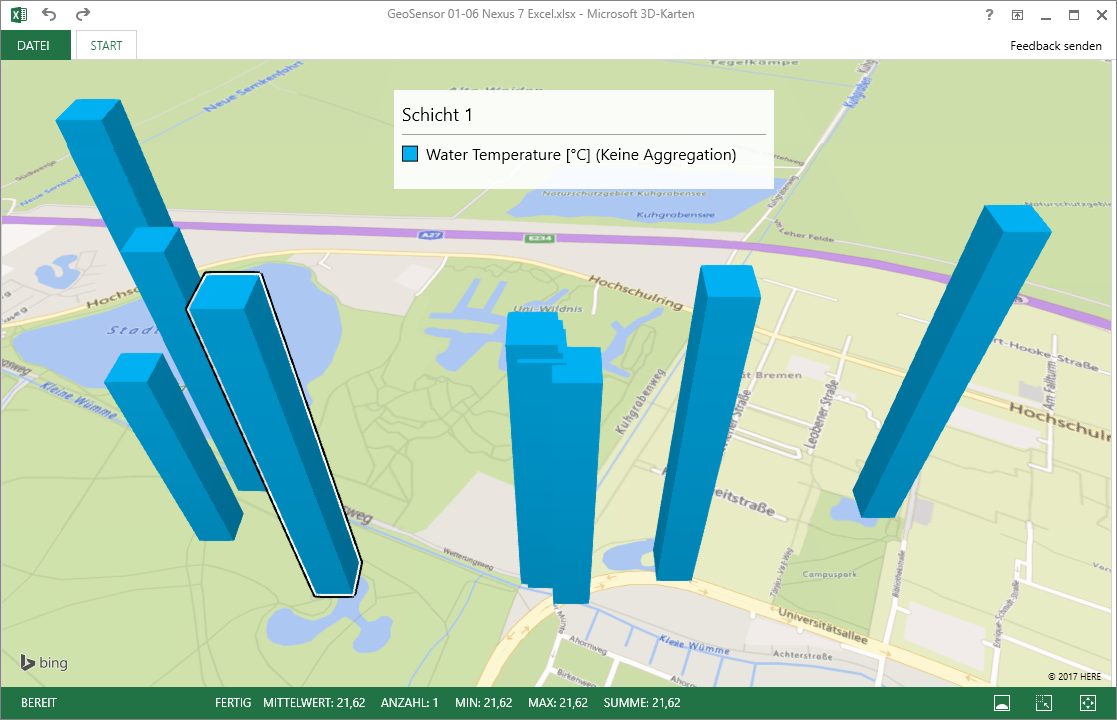
\includegraphics[width=1.0\textwidth]{src/excel_bar_graph.png}
\caption{Bar graph visualization of the field test data generated using Excel for Windows. Map data copyright 2017 HERE.}
\label{fig:excel_bar_graph}
\end{figure*}

\subsubsection{Matlab}
The version stored in Google Drive has been imported into Matlab R2017a on both the Windows 10 and the macOS 10.12 platform using a function generated by the graphical import tool and then plotted to a webmap (part of the Matlab Mapping Toolbox). The interactive webmap created by this procedure strongly resembles the map view included in the app. However, the data can then be analyzed further leveraging Matlabs manifold capabilities. A Matlab webmap generated using map data from OpenStreetMaps is shown in figure \ref{fig:matlab_webmap}. A Matlab Live Script (For Matlab R2017a including the Mapping toolbox) generating this map and the respective measure data can be found in the digital appendix.
\begin{figure*}[ht]
\centering
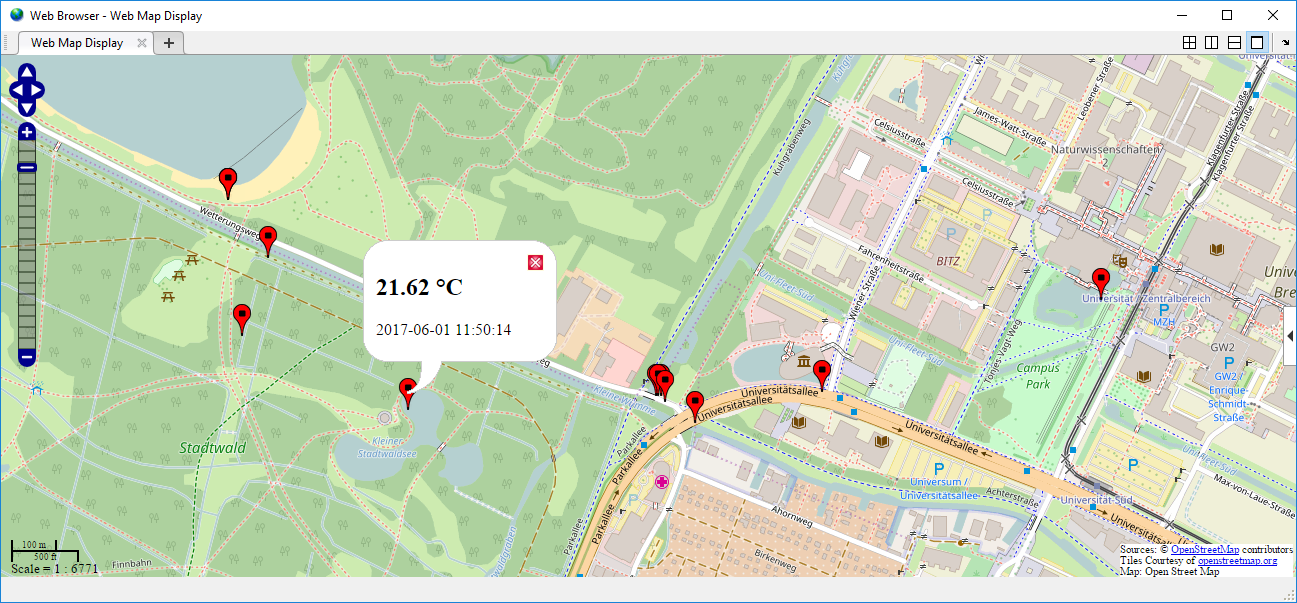
\includegraphics[width=1.0\textwidth]{src/matlab_webmap.png}
\caption{Visualisation of field test data on a Matlab webmap}
\label{fig:matlab_webmap}
\end{figure*}